% This tex file is available under a
% Creative Commons Attribution-Share Alike license (CC BY-SA 2.0).
% http://creativecommons.org/licenses/by-sa/2.0/
% Copyright © 2013 Rodrigo Hausen
\documentclass{beamer}
\usepackage[utf8]{inputenc}
\usepackage{lmodern}
\usepackage[T1]{fontenc}
\usepackage[portuguese,brazil]{babel}
\usepackage{url}
\usepackage{listings}
\usepackage{color}
\usepackage{textcomp}
\usepackage{pdfpages}
\usepackage{fancyvrb}
\usepackage{enumerate}
\usepackage{alltt}
\usepackage{array}
\usepackage{slashbox}
%\usepackage[pdf]{pstricks}
%\usepackage{auto-pst-pdf}
%\usepackage{icomma} % para vírgula decimal / decimal comma
\definecolor{listinggray}{gray}{0.9}
\definecolor{mediumgray}{rgb}{0.6,0.6,0.6}
\definecolor{lbcolor}{rgb}{0.9,0.9,0.9}
\lstset{
    backgroundcolor=\color{lbcolor},
    tabsize=4,
    rulecolor=,
    basicstyle=\scriptsize,
    upquote=true,
    aboveskip={1.5\baselineskip},
    columns=fixed,
    showstringspaces=false,
    extendedchars=true,
    breaklines=true,
    prebreak = \raisebox{0ex}[0ex][0ex]{\ensuremath{\hookleftarrow}},
    frame=single,
    showtabs=false,
    showspaces=false,
    showstringspaces=false,
    identifierstyle=\ttfamily,
    keywordstyle=\color[rgb]{0,0,1},
    commentstyle=\color[rgb]{0.133,0.545,0.133},
    stringstyle=\color[rgb]{0.627,0.126,0.941},
}
\definecolor{pinegreen}{RGB}{0,139,114}
\definecolor{pgr}{RGB}{0,139,114}

\definecolor{aquamarine}{RGB}{0,181,190}
\definecolor{aqm}{RGB}{0,181,190}

\definecolor{skyblue}{RGB}{100,227,251}
\definecolor{skb}{RGB}{100,227,251}

\definecolor{pnk}{RGB}{255,150,150}

\newcommand{\comment}[1]{{\color{structure.fg!70!white}\footnotesize #1}}

\newcommand{\WD}[1]{\fbox{#1}\hspace{-0.5pt}}
\newcommand{\FWD}[1]{%
\fbox{%
\vbox to 10pt{\vfil%
\hbox to 0.8cm{\hfill#1\hfill}%
\vfil}%
}\hspace{-0.5pt}%
}

\def\A{\texttt{A}}
\def\B{\texttt{B}}
\def\C{\texttt{C}}
\def\D{\texttt{D}}
\def\E{\texttt{E}}
\def\F{\texttt{F}}

\usetheme{Boadilla}
%\usetheme{umbc2}
\usefonttheme{structuresmallcapsserif}
\usecolortheme{seahorse}

\title{Aula 13: Circuitos Digitais Sequenciais -- Flip-flops}
\subtitle{Circuitos Digitais}
\author{Rodrigo Hausen}
\institute{CMCC -- UFABC} 
\date{11 e 13 de março de 2013}

\newcommand{\Not}[1]{\overline{#1}}
\def\And{\,}

\begin{document}

\begin{frame}
\maketitle

\vspace{-1cm}

\begin{center}
\url{http://compscinet.org/circuitos}
\end{center}

\end{frame}

%%%%%%%%%%%%%%%%%%%%%%%%%%%%%%%%%%%%%%%%%%%%%%%%%
\begin{frame}
\frametitle{Relembrando Latches}

\textbf{Latch do tipo $R$-$S$} (Reset-Set)

\begin{center}
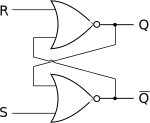
\includegraphics{images/latchRS_circuit}
\hspace{6ex}
\raisebox{40pt}{\Huge$=$}
\hspace{6ex}
\includegraphics{images/latchRS_blackbox}\\

\vspace{12pt}


\begin{tabular}{cc||ccl}
$R$ & $S$ & $Q_i$ & $\Not{Q_i}$ \\
\cline{1-4}
 1  &  0  &   0   &     1       & (reset $Q$) \\
 0  &  1  &   1   &     0       & (set $Q$) \\
 0  &  0  & $Q_{i-1}$ & $\Not{Q_{i-1}}$ & (mantém $Q$) \\
 1  &  1  &   X   &     X       & (estado proibido)
\end{tabular}
\end{center}
\end{frame}

%%%%%%%%%%%%%%%%%%%%%%%%%%%%%%%%%%%%%%%%%%%%%%%%%
\begin{frame}
\frametitle{Relembrando Latches}

\textbf{Latch do tipo $\Not{S}$-$\Not{R}$} (set-reset com entradas ativas em nível baixo)

\begin{center}
\includegraphics{images/latchRSnand_circuit}
\hspace{6ex}
\raisebox{40pt}{\Huge$=$}
\hspace{6ex}
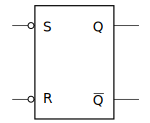
\includegraphics{images/latchRSnand_blackbox}\\

\vspace{12pt}

\begin{tabular}{cc||ccl}
$\Not{S}$ & $\Not{R}$ & $Q_i$ & $\Not{Q_i}$ \\
\cline{1-4}
 1  &  0  &   0   &     1       & (reset $Q$) \\
 0  &  1  &   1   &     0       & (set $Q$) \\
 1  &  1  & $Q_{i-1}$ & $\Not{Q_{i-1}}$ & (mantém $Q$) \\
 0  &  0  &   X   &     X       & (estado proibido)
\end{tabular}
\end{center}
\end{frame}

%%%%%%%%%%%%%%%%%%%%%%%%%%%%%%%%%%%%%%%%%%%%%%%%%
\begin{frame}
\frametitle{Relembrando Latches}

\textbf{Circuito de Habilitação} (enable)

\begin{center}
\includegraphics{images/enable_circuit}
\end{center}

\end{frame}

%%%%%%%%%%%%%%%%%%%%%%%%%%%%%%%%%%%%%%%%%%%%%%%%%
\begin{frame}
\frametitle{Relembrando Latches}

\vspace{-6pt}

\textbf{Latch do tipo $S$-$R$ com enable}

\begin{center}
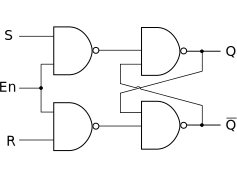
\includegraphics[scale=0.8]{images/latchRSnandEnable_circuit}%
%
\raisebox{60pt}{\Huge=}%
%
\raisebox{12pt}{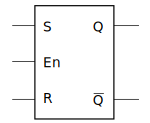
\includegraphics{images/latchRSenable_blackbox}}%

\begin{tabular}{ccc||cl}
$En$ & $S$ & $R$ & $Q_i$ \\
\cline{1-4}
 1   &  0  &  1  &   0  & (reseta $Q$) \\
 1   &  1  &  0  &   1  & (seta $Q$) \\
 1   &  0  &  0  & $Q_{i-1}$  & (mantém $Q$) \\
 1   &  1  &  1  & X  & (proibido) \\
 0   &  ?  &  ?  & $Q_{i-1}$  & (mantém $Q$, não importa $R$ nem $S$) \\
\end{tabular}
\end{center}
\end{frame}

%%%%%%%%%%%%%%%%%%%%%%%%%%%%%%%%%%%%%%%%%%%%%%%%%
\begin{frame}
\frametitle{Relembrando Latches}

\textbf{Latch do tipo $D$ (data)}

\begin{center}

\hspace*{\fill}
\includegraphics{images/latchD}%
\hspace*{\fill}%
\raisebox{40pt}{\Huge=}%
\hspace*{\fill}%
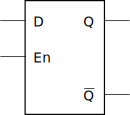
\includegraphics{images/latchD_blackbox}%
\hspace*{\fill}

\vspace{12pt}

\begin{tabular}{cc||cl}
$D$ & $En$ & $Q_i$  \\
\cline{1-3}
 0  &   1  &   0   & (reset) \\
 1  &   1  &   1   & (set) \\
 ?  &   0  & $Q_{i-1}$ & (mantém, sem se importar com $D$) \\
\end{tabular}
\end{center}

\end{frame}

%%%%%%%%%%%%%%%%%%%%%%%%%%%%%%%%%%%%%%%%%%%%%%%%%
\begin{frame}
\frametitle{Flip-flops}

\begin{itemize}
\item Analise o comportamento do circuito abaixo.
\end{itemize}

\begin{center}
\only<1-2>{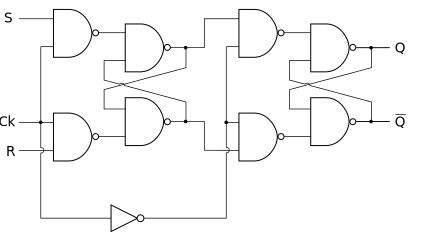
\includegraphics{images/flipflopRS0}}%
\only<3>{\includegraphics{images/flipflopRS}}%
\only<4-5>{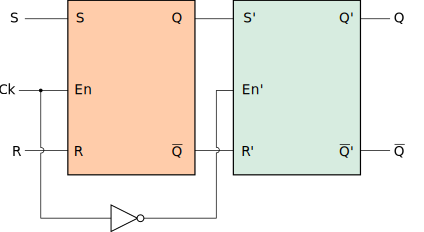
\includegraphics{images/flipflopRS2}}%
\end{center}
\vspace{-6pt}
\only<1,3-4>{\phantom{(Primeiro conselho: ``{\color{red!60!black}\textbf{DON'T PANIC}}'')}}
\only<2>{(Primeiro conselho: ``{\color{red!60!black}\textbf{DON'T PANIC}}'')}
\only<5>{(Segundo conselho: use um diagrama de forma de onda)}
\end{frame}

%%%%%%%%%%%%%%%%%%%%%%%%%%%%%%%%%%%%%%%%%%%%%%%%%
\begin{frame}
\frametitle{Flip-flop S-R: Diagrama de Forma de Onda}

\hspace*{\fill}%
\includegraphics[scale=0.9]{images/waveformFlipflopRS}%
\hspace*{\fill}%

\vspace{-6pt}

\begin{center}
Sensível à borda de descida do clock!
\end{center}


\end{frame}

%%%%%%%%%%%%%%%%%%%%%%%%%%%%%%%%%%%%%%%%%%%%%%%%%
\begin{frame}
\frametitle{Flip-flop S-R}

\textbf{Flip-flop S-R sensível à borda de descida do clock} (borda negativa)

\begin{center}
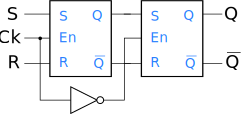
\includegraphics{images/flipflopRS_circuit}
\hspace{2ex}\pause
\raisebox{50pt}{\Huge$=$}\pause
\hspace{2ex}
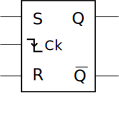
\includegraphics{images/flipflopRS_blackbox}

\pause

\vspace{12pt}

\begin{tabular}{ccc||cl}
$S$ & $R$ &        $Ck$       & $Q_i$ \\
\cline{1-4}
 0  &  0  &        $?$        & $Q_{i-1}$  & (mantem $Q$) \\
 0  &  1  &  1$\rightarrow$0  &     0      & (reset $Q$) \\
 1  &  0  &  1$\rightarrow$0  &     1      & (set $Q$) \\
 1  &  1  &  1$\rightarrow$0  &     X  & (proibido) \\
\end{tabular}
\end{center}

\end{frame}

%%%%%%%%%%%%%%%%%%%%%%%%%%%%%%%%%%%%%%%%%%%%%%%%%
\begin{frame}
\frametitle{Flip-flop S-R}

\textbf{Flip-flop S-R sensível à borda de subida do clock} (borda positiva)

\begin{center}
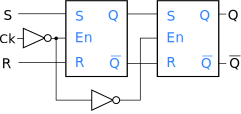
\includegraphics{images/flipflopRSpos_circuit}
\hspace{2ex}
\raisebox{50pt}{\Huge$=$}
\hspace{2ex}
\includegraphics{images/flipflopRSpos_blackbox}

\vspace{12pt}

\begin{tabular}{ccc||cl}
$S$ & $R$ &        $Ck$       & $Q_i$ \\
\cline{1-4}
 0  &  0  &        $?$        & $Q_{i-1}$  & (mantem $Q$) \\
 0  &  1  &  0$\rightarrow$1  &     0      & (reset $Q$) \\
 1  &  0  &  0$\rightarrow$1  &     1      & (set $Q$) \\
 1  &  1  &  0$\rightarrow$1  &     X  & (proibido) \\
\end{tabular}
\end{center}

\end{frame}

%%%%%%%%%%%%%%%%%%%%%%%%%%%%%%%%%%%%%%%%%%%%%%%%%
\begin{frame}
\frametitle{Flip-flop S-R: notação}

\textbf{Atenção:} o livro do Floyd adota notação diferente para os flip-flops

\begin{center}
\begin{tabular}{ccc}
sens. à borda      &    Floyd   & slides \\[12pt]
\raisebox{50pt}{subida (positiva)}  &   \includegraphics{images/flipflopRSpos_floyd}         & \includegraphics{images/flipflopRSpos_blackbox} \\
\raisebox{50pt}{descida (negativa)} &   \includegraphics{images/flipflopRS_floyd}            & 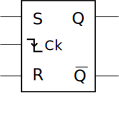
\includegraphics{images/flipflopRS_blackbox}
\end{tabular}
\end{center}

\end{frame}


%%%%%%%%%%%%%%%%%%%%%%%%%%%%%%%%%%%%%%%%%%%%%%%%%
\begin{frame}
\frametitle{Flip-flop S-R: Entradas Proibidas}

\begin{itemize}
\item Assim como o \emph{latch} S-R e o \emph{latch} S-R com enable, o
flip-flop S-R não admite que ambas as entradas $S$ e $R$ estejam
ativas quando a borda de descida/subida do clock é detectada.
\pause
\begin{itemize}
\item para um flip-flop S-R sensível à borda de subida, se $S = 1$,
$R = 1$ e $Ck$ fizer a transição 0$\rightarrow$1, o circuito
entra em oscilação descontrolada
\end{itemize}
\pause
\item \textbf{Solução 1}: evitar que ambas as entradas fiquem em $1$,
fazendo um \textbf{flip-flop D}

\begin{center}
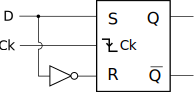
\includegraphics{images/flipflopD_circuit}%
\hspace{3ex}\pause%
\raisebox{40pt}{\Huge$=$}\pause%
\hspace{3ex}%
\includegraphics{images/flipflopD_blackbox}
\end{center}

\end{itemize}

\end{frame}

%%%%%%%%%%%%%%%%%%%%%%%%%%%%%%%%%%%%%%%%%%%%%%%%%
\begin{frame}
\frametitle{Flip-flop D: memória síncrona de 1 bit}

Flip-flop D sensível à borda de descida.

\begin{center}
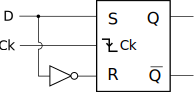
\includegraphics{images/flipflopD_circuit}%
\hspace{3ex}%
\raisebox{40pt}{\Huge$=$}%
\hspace{3ex}%
\includegraphics{images/flipflopD_blackbox}

\vspace{12pt}

\begin{tabular}{cc||cl}
 $D$ &        $Ck$       & $Q_i$ \\
\cline{1-3}
  0  &  1$\rightarrow$0  &     0      & (reset = armazena 0) \\
  1  &  1$\rightarrow$0  &     1      & (set = armazena 1) \\
\end{tabular}
\end{center}

\pause

\vspace{6pt}

\begin{minipage}{0.42\textwidth}
Se o circuito for feito com um flip-flop S-R sensível à borda de subida, o
flip-flip D resultante terá tabela verdade:
\end{minipage}
\hfill
\begin{minipage}{0.55\textwidth}
\begin{tabular}{cc||cl}
 $D$ &        $Ck$       & $Q_i$ \\
\cline{1-3}
  0  &  0$\rightarrow$1  &     0      & (reset = armazena 0) \\
  1  &  0$\rightarrow$1  &     1      & (set = armazena 1) \\
\end{tabular}
\end{minipage}

\end{frame}

%%%%%%%%%%%%%%%%%%%%%%%%%%%%%%%%%%%%%%%%%%%%%%%%%
\begin{frame}
\frametitle{Flip-flop J-K}

\textbf{Solução 2} para o problema do estado proibido no flip-flop S-R:\\
\begin{itemize}
\item no flip-flop D, perdemos uma entrada separada
\item solução sem perder entradas:
\end{itemize}
\hspace*{\fill}%
\only<1>{\includegraphics[scale=0.85]{images/flipflopJK0}}%
\only<2>{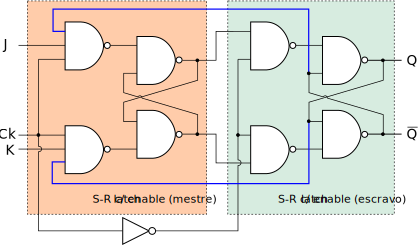
\includegraphics[scale=0.85]{images/flipflopJK}}%
\hspace*{\fill}%

\end{frame}

%%%%%%%%%%%%%%%%%%%%%%%%%%%%%%%%%%%%%%%%%%%%%%%%%
\begin{frame}
\frametitle{Flip-flop J-K}

\textbf{Flip-flop J-K} (Jump-Kill): flip-flop S-R com inclusão de duas realimentações.

\vspace{12pt}

\hspace*{\fill}%
\includegraphics[scale=0.85]{images/flipflopJK2}
\hspace*{\fill}%

\vspace{6pt}

Análise: ver arquivo \url{circuits/flipflopJK.circ}
\end{frame}

%%%%%%%%%%%%%%%%%%%%%%%%%%%%%%%%%%%%%%%%%%%%%%%%%
\begin{frame}
\frametitle{Flip-flop J-K: Resumo}

\begin{center}
\includegraphics[width=0.5\textwidth]{images/flipflopJK2}%
\hspace{3ex}\pause%
\raisebox{40pt}{\Huge$=$}\pause%
\hspace{3ex}%
\includegraphics{images/flipflopJK_blackbox}

\vspace{12pt}

\pause

\begin{tabular}{ccc||ccl}
$J$ & $K$ &        $Ck$       & $Q_i$           & $\Not{Q_i}$ \\[4pt]
\cline{1-5}
    &     &                   &                 &    \\[-8pt]
 0  &  0  &        $?$        & $Q_{i-1}$       & $\Not{Q_{i-1}}$ & (mantem) \\
 0  &  1  &  0$\rightarrow$1  &     0           &       1         & (kill = reset) \\
 1  &  0  &  0$\rightarrow$1  &     1           &       0         & (jump = set) \\ \pause
 1  &  1  &  0$\rightarrow$1  & $\Not{Q_{i-1}}$ & $Q_{i-1}$       & (inverte) \\
\end{tabular}

\end{center}

\end{frame}

%%%%%%%%%%%%%%%%%%%%%%%%%%%%%%%%%%%%%%%%%%%%%%%%%
\begin{frame}
\frametitle{Flip-flop J-K: Aplicação}

O que faz o circuito abaixo?
\begin{itemize}
\item entrada: $Ck$
\item saídas: $a_2, a_1, a_0$
\end{itemize}
Suponha que o estado inicial de cada saída é $0$.

\vspace{12pt}

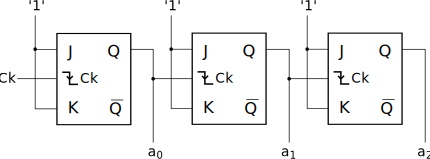
\includegraphics[width=\textwidth]{images/counter}

(Solução na lousa) \pause É um contador de $3$ bits!

\end{frame}

%%%%%%%%%%%%%%%%%%%%%%%%%%%%%%%%%%%%%%%%%%%%%%%%%
\begin{frame}
\frametitle{Para Casa}

\begin{itemize}
\item Leia:\\
{\footnotesize
\hspace{-2ex}	\url{http://www.play-hookey.com/digital/sequential/rs_nand_flip-flop.html}\\
\hspace{-2ex}	\url{http://www.play-hookey.com/digital/sequential/d_nand_flip-flop.html}\\
\hspace{-2ex}	\url{http://www.play-hookey.com/digital/sequential/jk_nand_flip-flop.html}\\
}
\item Exercícios do livro do Floyd: autotestes 5--8, problemas 8--13 e 15.
\item Se necessário, ler seção 7-2
\item \textbf{Para casa:} desenhar o diagrama completo do circuito do pisca-pisca de natal
com 16 níveis (Aula 11), recebendo o clock como entrada. Você possui os seguintes componentes:
um decodificador $4 \times 16$ e flip-flops J-K.
\pause
\item So long, and thanks for all the fish!
\end{itemize}
\end{frame}

\end{document}
